\documentclass[crop, tikz]{standalone}

\usetikzlibrary{patterns, decorations.pathreplacing}

\begin{document}
    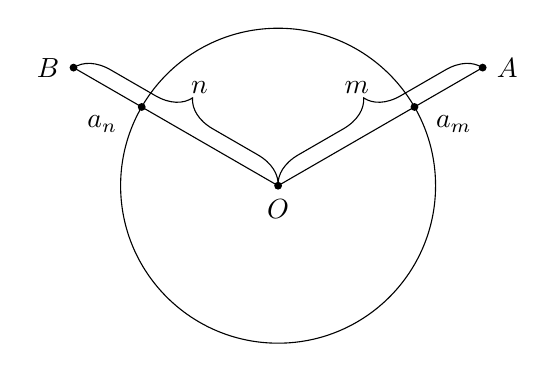
\begin{tikzpicture}[scale=1]
        \draw (0, 0) circle (2) node[circle, fill, inner sep=1pt, label=below:$O$](O){};
        %\draw (0, 0) circle (3);
        
        \draw (0, 0) -- (2.598, 1.5) node[circle, fill, inner sep=1pt, label=right:$A$](A){};
        \draw (1.732, 1) node[circle, fill, inner sep=1pt, label={[xshift=0.5cm, yshift=-0.5cm]$a_m$}](am){};
        
        \draw (0, 0) -- (-2.598, 1.5) node[circle, fill, inner sep=1pt, label=left:$B$](B){};
        \draw (-1.732, 1) node[circle, fill, inner sep=1pt, label={[xshift=-0.5cm, yshift=-0.5cm]$a_n$}](an){};
        
        \draw[
            decorate,
            decoration={
                brace,
                amplitude=12pt
            }
        ] (0, 0) -- (2.598, 1.5) node[black, midway, yshift=0.5cm, xshift=-0.3cm]{$m$};
        
        \draw[
            decorate,
            decoration={
                brace,
                mirror,
                amplitude=12pt
            }
        ] (0, 0) -- (-2.598, 1.5) node[black, midway, yshift=0.5cm, xshift=0.3cm]{$n$};
    \end{tikzpicture}
\end{document}